\subsubsection{Estensione D: Annullamento della Controproposta nella Finestra di Conferma}

Nel caso in cui, all’interno della finestra di conferma, l’agente scelga di annullare l’invio della controproposta, il sistema non procede con il salvataggio dei dati né con l’invio della notifica all’utente.

\subsubsection{Comportamento del Sistema}
Se l’agente clicca su \textbf{“Annulla”} invece di confermare l’operazione, la finestra di dialogo viene chiusa e il flusso ritorna al punto 6 dello scenario principale, consentendo la modifica o la revisione del prezzo proposto.  

Questa interazione segue il principio del \textbf{controllo da parte dell’utente} \cite{nielsen1995}, garantendo la possibilità di interrompere o modificare l’azione prima della sua esecuzione definitiva.
\begin{figure}[H]
	\centering
	\begin{tikzpicture}[node distance=1.5cm and 1cm, auto]
		% Nodo per la finestra di conferma
		\node (img1) {
			\begin{tabular}{c}
				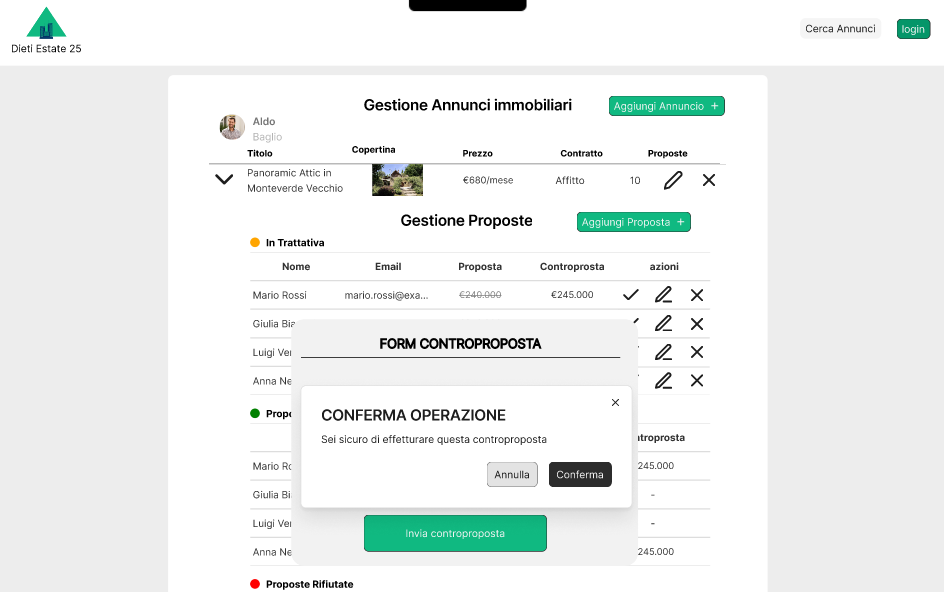
\includegraphics[width=0.7\textwidth]{Immagini/Mockup/controproposte/Extensions D/FinestraConfermaControproposta.png} \\
				Cockburn: step 9.D
			\end{tabular}
		};

		% Nodo per l'azione di annullamento e ritorno alla schermata di modifica
		\node (img2) [below=of img1] {
			\begin{tabular}{c}
				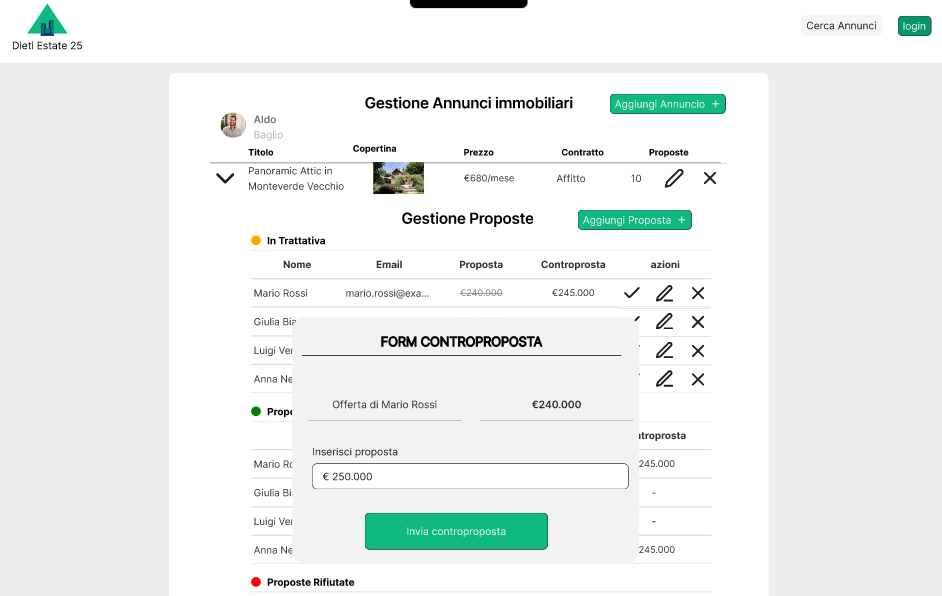
\includegraphics[width=0.7\textwidth]{Immagini/Mockup/controproposte/Extensions D/SchermataContropropostaAnnullata.png} \\
				Cockburn: ritorno al punto 6
			\end{tabular}
		};

		% Disegna la freccia tra i due step
		\draw[->, thick] (img1) -- (img2);

	\end{tikzpicture}
	\caption{Mockup: Extension D della tabella di Cockburn del caso d'uso: Fare una controproposta a un'offerta.}
	\label{fig:tikz_flow_extensionD}
\end{figure}

\newpage


